\documentclass[10pt]{exam}
\usepackage[hon]{template-for-exam}
\usepackage{tikz}

\title{Multi-Force Circular Problem (Consolidation)}
\author{Rohrbach}
\date{\today}

\begin{document}
\maketitle

\noindent
A roller coaster car of mass 600~kg goes around a loop of radius 8 meters with an (assumed constant) speed of 9~m/s.  

\vspace{2em}

\begin{parts}
  \part 
    Find the normal force of the track on the coaster at the bottom of the loop.

    \vspace{1em}

    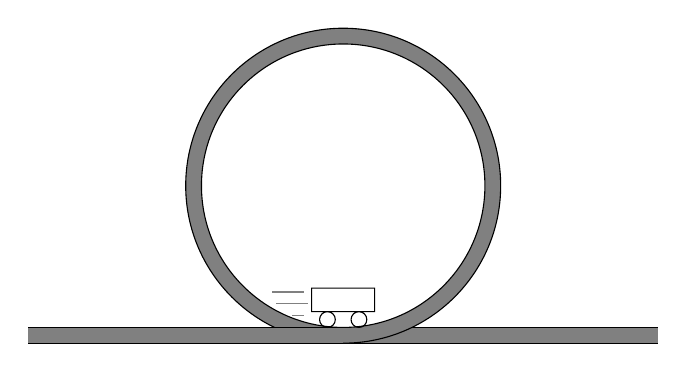
\begin{tikzpicture}

      \fill[gray] (4,0) rectangle ++(4,0.2);
      \draw (4,0) -- ++(4,0);
      \draw (4,0.2) -- ++(4,0);
    
      \coordinate (c) at (4,2);
      \draw[fill=gray] (c) circle (2);
      \draw[fill=white] (c) circle (1.8);
    
      \fill[gray] (0,0) rectangle ++(4,0.2);
      \draw (0,0) -- ++(4,0);
      \draw (0,0.2) -- ++(4,0);
    
      \draw (4,0) +(-0.2,0.3) circle (0.1)
                  +(0.2,0.3)  circle (0.1)
                  ++(-0.4,0.4) rectangle ++(0.8,0.3);

      \draw[thin,gray] (3.5,0.65) -- +(-0.4,0)
                  ++(0.05,-.15) -- +(-0.4,0)
                  ++(-0.05,-.15) -- +(-0.15,0);
    
    
    \end{tikzpicture}

    \vs

  \part
    Find the normal force of the track on the coaster at the top of the loop.

    \vspace{1em}

    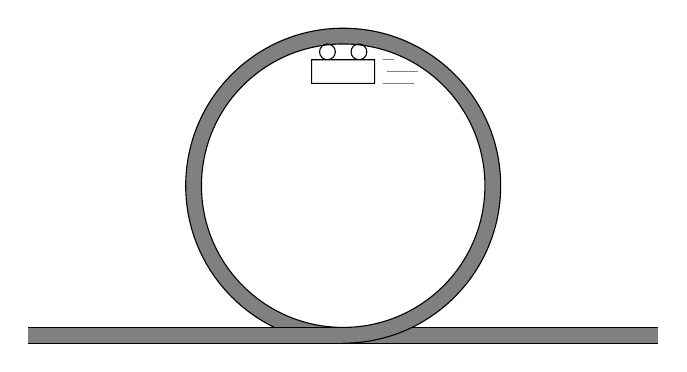
\begin{tikzpicture}

      \fill[gray] (4,0) rectangle ++(4,0.2);
      \draw (4,0) -- ++(4,0);
      \draw (4,0.2) -- ++(4,0);
    
      \coordinate (c) at (4,2);
      \draw[fill=gray] (c) circle (2);
      \draw[fill=white] (c) circle (1.8);
    
      \fill[gray] (0,0) rectangle ++(4,0.2);
      \draw (0,0) -- ++(4,0);
      \draw (0,0.2) -- ++(4,0);
    
      \draw (4,4) +(-0.2,-0.3) circle (0.1)
                  +(0.2,-0.3)  circle (0.1)
                  ++(-0.4,-0.4) rectangle ++(0.8,-0.3);

      \draw[thin,gray] (4.5,3.3) -- +(0.4,0)
                  ++(0.05,.15) -- +(0.4,0)
                  ++(-0.05,.15) -- +(0.15,0);
    
    
    \end{tikzpicture}

    \vs

  \part
    What is the minimum speed the car needs to not fall off at the top of the loop? 

    \vspace{1em}

    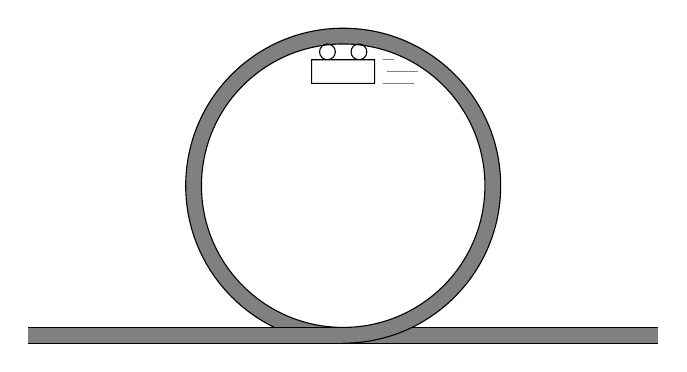
\begin{tikzpicture}

      \fill[gray] (4,0) rectangle ++(4,0.2);
      \draw (4,0) -- ++(4,0);
      \draw (4,0.2) -- ++(4,0);
    
      \coordinate (c) at (4,2);
      \draw[fill=gray] (c) circle (2);
      \draw[fill=white] (c) circle (1.8);
    
      \fill[gray] (0,0) rectangle ++(4,0.2);
      \draw (0,0) -- ++(4,0);
      \draw (0,0.2) -- ++(4,0);
    
      \draw (4,4) +(-0.2,-0.3) circle (0.1)
                  +(0.2,-0.3)  circle (0.1)
                  ++(-0.4,-0.4) rectangle ++(0.8,-0.3);

      \draw[thin,gray] (4.5,3.3) -- +(0.4,0)
                  ++(0.05,.15) -- +(0.4,0)
                  ++(-0.05,.15) -- +(0.15,0);
    
    
    \end{tikzpicture}


    \vs


\end{parts}





\end{document}